\documentclass[a4paper, 12pt]{article}
\usepackage[T2A]{fontenc}
\usepackage[utf8]{inputenc}
\usepackage[russian]{babel}
\usepackage{amsmath}
\usepackage{indentfirst}
\usepackage{graphicx}
\usepackage{pgfplots}
\usepackage[top=2cm, bottom=2cm, left=3cm, right=1cm]{geometry}

\newcommand{\Pra}{\mathbf{Pr}}
\newcommand{\Gra}{\mathbf{Gr}}
\newcommand{\der}[2]{\frac{\partial {#1}}{\partial {#2}}}
\newcommand{\dder}[2]{\frac{\partial^2 {#1}}{\partial {#2}^2}}
\newcommand{\psp}[2]{\psi_{\mathring{#1}}^{#2}}

\begin{document}
  \begin{titlepage}
    \begin{center} %% ПО ЦЕНТРУ
      \bfseries

      {\Large Белорусский государственный университет}

      \vspace{96pt}

      {\large Факультет прикладной математики и информатики}

      \vspace{72pt}

      {\large Кафедра вычислительной математики}

      \vspace{96pt}

      Отчет по лабораторной работе

      \vspace{24pt}

      Вариант №4

      \vspace{24pt}

      {\Large Вычислительный эксперимент в конвекции}

    \end{center}

    \vspace{120pt}

    \begin{flushright}
      \begin{tabular}{rl}
        Подготовили: & Д.\,Г. Борисевич \\
                     & И.\,И. Демух \\
                     & В.\,A. Сидоров \\
                     &студенты 5 курса 5 группы\\
        Преподаватель: & В.\,К. Полевиков \\
      \end{tabular}
    \end{flushright}

    \vfill

    \begin{center}
      \bfseries
      Минск, 2016
    \end{center}
  \end{titlepage}

  \section{Постановка задачи}
    Решить задачу естественной конвекции несжимаемой жидкости в двумерной
    области.
    \begin{itemize}
      \item Монтонная разностная схема порядка $O(h)$
      \item Граничные условия:
        \begin{center}
        \begin{tikzpicture}
            \Large
            \draw (0,0)
            -- (10,0) node[midway,below] {$T=0$} node[below] {$1$}
            -- (10,10) node[midway,right] {$T=sin\pi y$}
            -- (0,10) node[midway,above] {$T=0$} node[left] {$1$}
            -- (0,0) node[midway,left] {$T=0$};
            \draw[->] (0,0) -- (0,11) node[left] {$Y$};
            \draw[->] (0,0) -- (11,0) node[right] {$X$};
        \end{tikzpicture}
        \end{center}
      \item Параметры: число Прандтля $\Pra=1.0$ и число Грасгофа
        $\Gra=[100;10000]$
    \end{itemize}

  \pagebreak

  \section{Уравнение конвекции}
    При составлении уравнения конвекции будем считать, что жидкость несжимаема и
    в объеме отсутсвуют источники тепла.

    Математическую модель процесса естественной конвекции обычно составляют из
    уравнения Навье-Стокса (закона сохранения количества движения):
    \begin{equation}
    \begin{gathered}
    \label{f1}
    \rho[\frac{\partial \overline v}{\partial t} + (\overline v \cdot \nabla)\overline v]=-\nabla p + \eta \nabla^2 \overline v + \frac{1}{3} \eta \nabla (\nabla \cdot \overline v) + \rho \overline g
    \end{gathered}
    \end{equation}

    уравнения неразрывности (закона сохранения массы):

    \begin{equation}
    \begin{gathered}
    \label{f2}
    \frac{\partial \rho}{\partial t} + \nabla \cdot (\rho \overline v) = 0
    \end{gathered}
    \end{equation}

    уравнения переноса тепла (закона сохранения энергии):

    \begin{equation}
    \begin{gathered}
    \label{f3}
    c \rho(\frac{\partial T}{\partial t} + \overline v \cdot \nabla T) = \lambda \nabla^2 T
    \end{gathered}
    \end{equation}

    и уравнение состояния:

    \begin{equation}
    \begin{gathered}
    \label{f4}
    \rho = \rho (T)
    \end{gathered}
    \end{equation}

    где неизвестные:

    \begin{enumerate}
    \item $ \vec v = (v_x, v_y, v_z)$
    \item $ p = p(x,y,z,t)$
    \item $ T = T(x,y,z,t)$
    \end{enumerate}

    и параметры:

    \begin{enumerate}
    \item динамическая вязкость $\eta$
    \item теплопроводность $\lambda$
    \item удельная теплоемкость $c$
    \item время $t$
    \item напряженность гравитационного поля $\overline g$
    \end{enumerate}

    Обратимся к приближению Буссинеска-Обербека:

    Все параметры --- константы

    $$ \rho = \rho_0 = \rho (T_0) = const $$

    $T_0$ выбираем в области задачи. Рассмотрим $\rho(T)$, раскладывая ее в ряд Тейлора в окрестности значения $T_0$

    $$\rho (T)) = \rho(T_0) + (T - T_0) \frac{\partial \rho(T_0))}{\partial T} + O(\left\lVert T - T_0 \right\rVert ^ 2)$$

    $\rho = \rho_0[1 - \beta(T - T_0)]$ --- приближение Буссинеска

    где $\beta = - \frac{1}{\rho_0} \frac{\partial \rho(T_0)}{\partial T}$ --- коэффициент теплового объемного расширения жидкости при $T=T_0$

    Главная идея приближения Буссинеска-Обербека заключается в том, что зависимость плотности от температуры учитывается лишь в члене с объемной силой тяжести $\rho \overline g$, а в остальных случаях полагают $\rho = \rho_0$. При таких допущениях система \eqref{f1}-\eqref{f4} примет вид:

    \begin{equation}
    \begin{gathered}
    \label{f5}
    \frac{\partial \overline v}{\partial t} + (\overline v \cdot \nabla)\overline v = -\frac{1}{\rho_0}\nabla p + \nu \nabla^2 \overline v + [1-\beta(T-T_0)]\overline g
    \end{gathered}
    \end{equation}

    \begin{equation}
    \begin{gathered}
    \label{f6}
    \nabla \cdot \overline v = 0
    \end{gathered}
    \end{equation}

    \begin{equation}
    \begin{gathered}
    \label{f7}
    \frac{\partial T}{\partial t} + \overline v \cdot \nabla T = a \nabla^2 T
    \end{gathered}
    \end{equation}

    В приближении Буссинеска \eqref{f1}-\eqref{f3} соответствует \eqref{f5}-\eqref{f7} если ${\beta |T-T_0| \ll 1}$.

    Обратим внимание на то, что функции тока и завихренности в этих уравнениях – это векторные величины. Запишем уравнения в скалярном виде.

    \begin{equation}
    \begin{gathered}
    \label{f8}
    \frac{\partial v_x}{\partial t} + v_x\frac{\partial v_x}{\partial x} + v_y\frac{\partial v_x}{\partial y} + v_z \frac{\partial v_x}{\partial z} = -\frac{1}{\rho_0}\frac{\partial p}{\partial x} + \nu \left(\frac{\partial^2 v_x}{\partial x^2} + \frac{\partial^2 v_x}{\partial y^2} + \frac{\partial^2 v_x}{\partial z^2}\right)\\
    \frac{\partial v_y}{\partial t} + v_x\frac{\partial v_y}{\partial x} + v_y\frac{\partial v_y}{\partial y} + v_z \frac{\partial v_y}{\partial z} = -\frac{1}{\rho_0}\frac{\partial p}{\partial y} + \nu \left(\frac{\partial^2 v_y}{\partial x^2} + \frac{\partial^2 v_y}{\partial y^2} + \frac{\partial^2 v_y}{\partial z^2}\right)\\
    \frac{\partial v_z}{\partial t} + v_x\frac{\partial v_z}{\partial x} + v_y\frac{\partial v_z}{\partial y} + v_z \frac{\partial v_z}{\partial z} = -\frac{1}{\rho_0}\frac{\partial p}{\partial z} + \nu \left(\frac{\partial^2 v_z}{\partial x^2} + \frac{\partial^2 v_z}{\partial y^2} + \frac{\partial^2 v_z}{\partial z^2}\right) - [1-\beta(T-T_0)]g
    \end{gathered}
    \end{equation}

    \begin{equation}
    \begin{gathered}
    \label{f9}
    \frac{\partial v_x}{\partial x} + \frac{\partial v_y}{\partial y} + \frac{\partial v_z}{\partial z} =0
    \end{gathered}
    \end{equation}

    \begin{equation}
    \begin{gathered}
    \label{f10}
    \frac{\partial T}{\partial t} + v_x \frac{\partial T}{\partial x}+ v_y \frac{\partial T}{\partial y} + v_z \frac{\partial T}{\partial z} = a(\frac{\partial^2 T}{\partial x^2} + \frac{\partial^2 T}{\partial y^2} + \frac{\partial^2 T}{\partial z^2})
    \end{gathered}
    \end{equation}

    \eqref{f8}-\eqref{f10} --- система уравнений в приближении Буссинеска в естественных переменных.

    Введем новые функции завихренности и тока: $(v,p) \to (\psi, \omega)$ и
    соотнесем их со старыми переменными:
    \begin{gather*}
      \omega = - \der{v_x}{y} + \der{v_y}{x}
      \\
      v_x = \der{\psi}{y}, \quad v_y = - \der{\psi}{x}
    \end{gather*}
    и друг с другом:
    $$
      \omega = - \dder{\psi}{x} - \dder{\psi}{y}
    $$

    Введем правую декартову прямоугольную систему координат $x,y,z$ направив
    $Oy$ противоположно вектору $g$. В этой системе координат получаем
    cледующее уравнение гравитационной конвекции:
    \begin{equation}
      \left\{
        \begin{aligned}
          &\der{T}{t} + \der{\psi}{y} \der{T}{x} - \der{\psi}{x} \der{T}{y} =
            a \left( \dder{T}{x} + \dder{T}{y} \right)
          \\
          &\dder{\psi}{x} + \dder{\psi}{y} + \omega = 0
          \\
          &\der{\omega}{t} + \der{\psi}{y} \der{\omega}{x} - \der{\psi}{x}
            \der{\omega}{y} = \nu \left(
              \dder{\omega}{x} + \dder{\omega}{y}
            \right) + \beta g \der{T}{x}
        \end{aligned}
      \right.\label{convection}
    \end{equation}

    Предположим, что размеры области характеризуются длиной $l$, а температурные
    условия на границе -- $\Delta T = T_1 - T_0$. Таким образом можно получить
    безразмерные переменные:
    \begin{gather*}
      x' = \frac{x}{l}, \quad y' = \frac{y}{l} \quad \Rightarrow \quad
        x = x' l, \quad y = y' l
      \\
      T'=\frac{T - T_0}{\Delta T} \quad \Rightarrow \quad
        T = T' \Delta T + T_0
    \end{gather*}

    Учитывая эти соотношения и опуская штрихи, получим безразмерную форму для
    уравнений гравитационной конвекции:
    $$
      \left\{
        \begin{aligned}
          &\der{\psi}{y} \der{T}{x} - \der{\psi}{x} \der{T}{y} = \frac{1}{\Pra}
            \left( \dder{T}{x} + \dder{T}{y} \right)
          \\
          &\dder{\psi}{x} + \dder{\psi}{y} + \omega = 0
          \\
          &\der{\psi}{y} \der{\omega}{x} - \der{\psi}{x} \der{\psi}{y} =
            \dder{\omega}{x} + \dder{\omega}{y} + \Gra \der{T}{x}
          \\
          &v_1 = \der{\psi}{y}, \quad v_2 = - \der{\psi}{x},
        \end{aligned}
      \right.
    $$
    где $\Pra = \frac{v}{a}, \quad \Gra = \frac{\beta g \Delta T l^{3}}{\nu}$ --
    числа Прандтля и Грасгофа.

    Итого окончательно, для стационарной задачи получаем следующую систему:
    \begin{equation}
      \begin{aligned}
        &\der{\psi}{y} \der{T}{x} - \der{\psi}{x} \der{T}{y} = \frac{1}{\Pra}
          \left( \dder{T}{x} + \dder{T}{y} \right)
        \\
        &\dder{\psi}{x} + \dder{\psi}{y} + \omega = 0
        \\
        &\der{\psi}{y} \der{\omega}{x} - \der{\psi}{x} \der{\psi}{y} =
          \dder{\omega}{x} + \dder{\omega}{y} + \Gra \der{T}{x}
      \end{aligned}\label{convection_final}
    \end{equation}
  \pagebreak

  \section{Разностная схема для уравнений конвекции}
    После введения безразмерных величин, область решения задачи представляет
    собой единичный квадрат. Построим равномерную сетку с длиной шага h по обоим
    направлениям и заменим исходную дифференциальную задачу
    \eqref{convection_final} разностной на построенной сетке узлов. Построенная
    сетка должна быть монотонной, то есть удовлетворять принципу максимума:
    \bigskip
    Пусть каждое уравнение РС может быть представлено в виде:
    \begin{equation}
      A(x) y(x) = \sum\limits_{\xi \in G'(x)} B(x,\xi)y(\xi) + F(x) \quad
        \forall x \in \Omega,\label{max_principle}
    \end{equation}
    где $y(x)$ -- искомая функция, $F(x)$ -- сеточная функция, $G(x)$ --
    шаблон схемы в узле $x$, $G'(x)$ -- окрестность узла $x$, $\Omega$ -- cетка.

    Тогда говорят, что РС удовлетворяет принципу максимума, если выполняются
    следующие условия
    \begin{gather*}
      A(x) > 0, \quad B(x,\xi) > 0 \quad \forall x \in \Omega, \xi \in G'(x)
      \\
      D(x) \equiv A(x)- \sum\limits_{\xi \in G'(x)} B(x,\xi) \geq 0
      \\
      \exists x_0 \in \Omega, D(x_0) > 0
    \end{gather*}

    Введем обозначения:
    \begin{gather*}
      f_{\mathring{x}} = \frac{f_{i+1,j} - f_{i-1,j}}{2 h}
      \\
      f_{\mathring{y}} = \frac{f_{i,j+1} - f_{i,j-1}}{2 h}
      \\
      f_{\overline{x}} = \frac{f_{i,j} - f_{i-1,j}}{h}
      \\
      f_{y} = \frac{f_{i,j+1} - f_{i,j}}{h}
      \\
      f_{x \overline{x}} = \frac{f_{i+1,j} - 2 f_{i,j} + f_{i-1,j}}{h^2}
      \\
      f^{+} = \left\{
        \begin{aligned}
          &f, \quad f > 0\\
          &0, \quad f \leq 0
        \end{aligned}
      \right.
      \\
      f^{-} = \left\{
        \begin{aligned}
          &f, \quad f < 0\\
          &0, \quad f \geq 0
        \end{aligned}
      \right.
    \end{gather*}

    Получим разностную схему:
    \begin{equation}
      \left\{
        \begin{aligned}
          &\left( \psp{y}{+} T_{\overline{x}} + \psp{y}{-} T_{x} \right) -
            \left( \psp{x}{+} T_{y} + \psp{x}{-} T_{\overline{y}} \right) =
            \frac{1}{\Pra}\left( T_{x \overline{x}} + T_{y \overline{y}} \right)
          \\
          &\psi_{x \overline{x}} + \psi_{y \overline{y}} + \omega = 0
          \\
          &\left(
            \psp{y}{+} \omega_{\overline{x}} + \psp{y}{-} \omega_{x}
          \right) - \left(
            \psp{x}{-} \omega_{\overline{y}} + \psp{x}{+} \omega_{y}
          \right) =
            \omega_{x \overline{x}} + \omega_{y \overline{y}} +
            \Gra T_{\mathring{x}}
        \end{aligned}
      \right.\label{diff_scheme}
    \end{equation}

    Каждая из этих трёх разностных схем является монотонной
    \eqref{max_principle} и аппроксимирует соответствующее дифференциальное
    уравнение с первым порядком точности. Построим итерационный процесс. Для
    каждого узла вычисляем значения температуры, функций тока и вихря по
    следующим расчетным формулам, которые следуют из \eqref{diff_scheme}:

    \begin{equation}
      \left\{
        \begin{aligned}
          &T_{i,j} =
            \frac{
              T_{i-1,j}\left(
                1 + h \Pra \psp{y}{+}
              \right) +
              T_{i,j-1}\left(
                1 - h \Pra \psp{x}{-}
              \right) +
              T_{i+1,j}\left(
                1 - h \Pra \psp{y}{-}
              \right) +
              T_{i,j+1}\left(
                1 + h \Pra \psp{x}{+}
              \right)
            }{4 + h \Pra \left(
              \psp{y}{+} + \psp{x}{+} - \psp{y}{-} - \psp{x}{-}
            \right)}
          \\
          &\psi_{i,j} = \frac{1}{4} \left(
            \psi_{i,j+1} + \psi_{i,j-1} + \psi_{i-1,j} + \psi_{i+1,j} +
            h^2 \omega_{i,j}
          \right)
          \\
          &\omega_{i,j} =
            \frac{
              \omega_{i+1, j} \left( 1 - h \psp{y}{-} \right) +
              \omega_{i-1, j} \left( 1 + h \psp{y}{+} \right) +
              \omega_{i, j-1} \left( 1 - h \psp{x}{-} \right) +
              \omega_{i, j+1} \left( 1 + h \psp{x}{+} \right) +
              h \Gra T_{\mathring{x}}
            }{4 + h \left(
              \psp{y}{+} + \psp{x}{+} - \psp{y}{-} - \psp{x}{-}
            \right)}
        \end{aligned}
      \right.
    \end{equation}
    
    Используя условия задачи для температуры, условия твердой стенки для тока и условия Вудса для завихренности 
    получаем следующие граничные условия:
    \begin{gather*}
      T_{i,0} = T_{0,j} = T_{i,N} = 0, \quad T_{N,j} = \sin (\pi j h)
      \\
      \psi_{i,0} = \psi_{0,j} = \psi_{i,N} = \psi_{N,j} = 0
      \\
      \omega_{i,0} = - \frac{1}{2} \omega_{i,1} - \frac{3}{h^2} \omega_{i,1}
      \\
      \omega_{0,j} = - \frac{1}{2} \omega_{1,j} - \frac{3}{h^2} \omega_{1,j}
      \\
      \omega_{i,N} = - \frac{1}{2} \omega_{i,N-1} - \frac{3}{h^2} \omega_{1,N-1}
      \\
      \omega_{N,j} = - \frac{1}{2} \omega_{N-1,j} - \frac{3}{h^2} \omega_{N-1,j}
      \\
    \end{gather*}

    Начально итерационное приближение:
    $$
      T_{i,j}^0 = \psi_{i,j}^{0} = \omega_{i,j}^{0} = 0
    $$

    Окончание итерационного процесса:
    $$
      \lVert T^{k+1} - T^k \rVert + 
      \lVert \psi^{k+1} - \psi^k \rVert +
      \lVert \omega^{k+1} - \omega^k \rVert 
      \leq \varepsilon
    $$

    , где $\varepsilon = h^2$.
  \pagebreak

  \section{Результаты}
    Была составлена программа, позволяющая моделировать задачу статической
    гравитационной конвекции.

    \bigskip
    Частное решение при $\Pra = 1, \Gra = 100, N = 20, h = 0.05$:
    \bigskip

    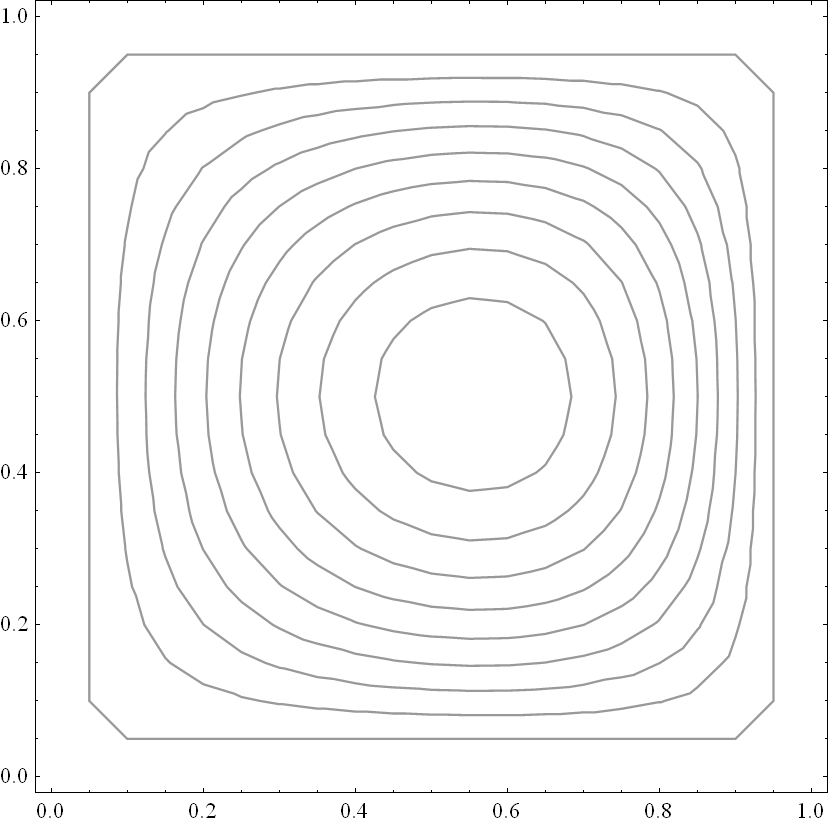
\includegraphics[scale=0.25]{images/psi_100.png}
    \qquad
    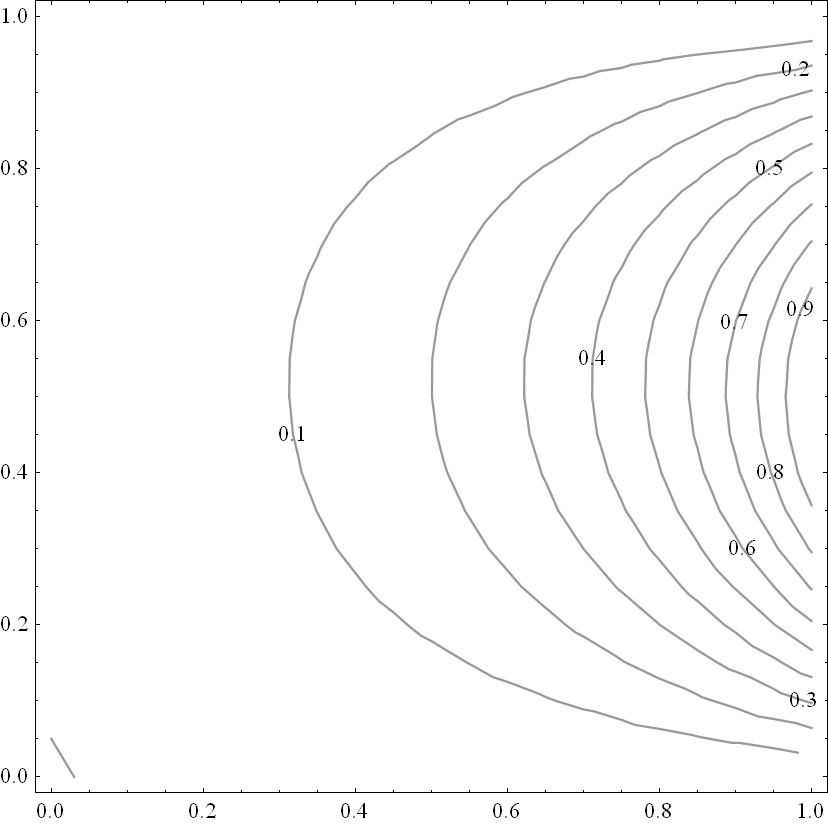
\includegraphics[scale=0.25]{images/t_100.png}

    \bigskip
    Частное решение при $\Pra = 1, \Gra = 10000, N = 20, h = 0.05$:
    \bigskip

    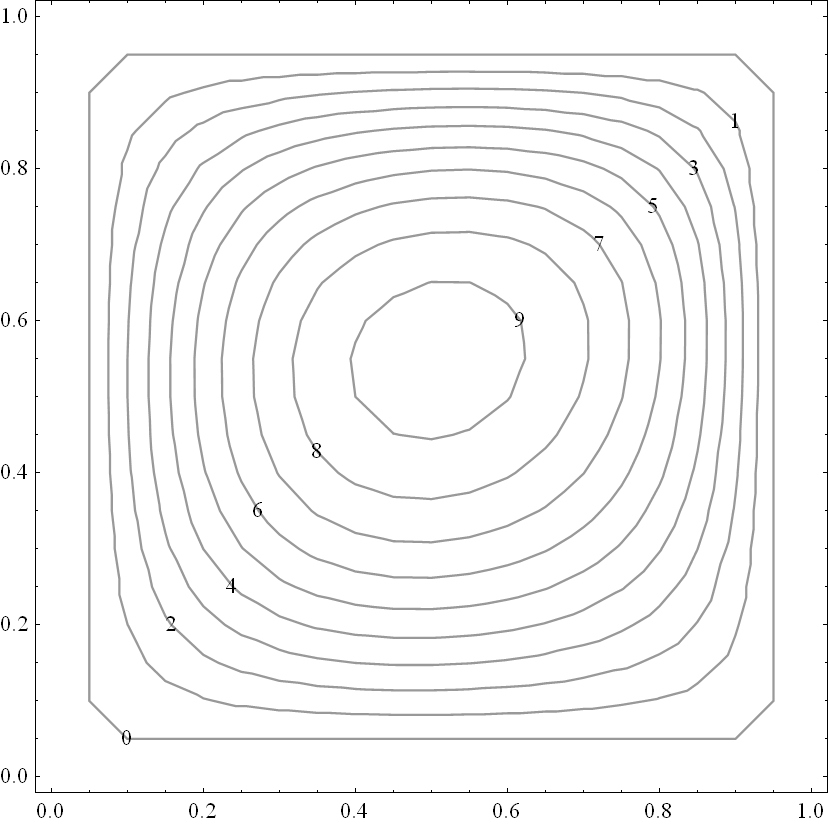
\includegraphics[scale=0.25]{images/psi_10k.png}
    \qquad
    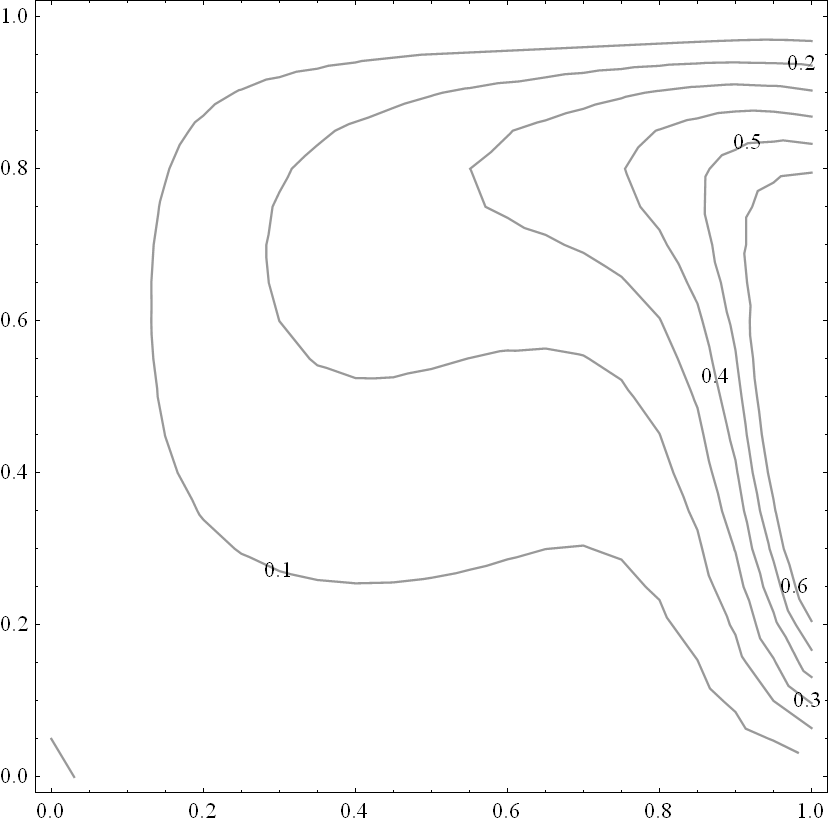
\includegraphics[scale=0.25]{images/t_10k.png}
\end{document}
